% Options for packages loaded elsewhere
% Options for packages loaded elsewhere
\PassOptionsToPackage{unicode}{hyperref}
\PassOptionsToPackage{hyphens}{url}
%
\documentclass[
  ignorenonframetext,
  aspectratio=169,
  russian,
]{beamer}
\newif\ifbibliography
\usepackage{pgfpages}
\setbeamertemplate{caption}[numbered]
\setbeamertemplate{caption label separator}{: }
\setbeamercolor{caption name}{fg=normal text.fg}
\beamertemplatenavigationsymbolshorizontal
% remove section numbering
\setbeamertemplate{part page}{
  \centering
  \begin{beamercolorbox}[sep=16pt,center]{part title}
    \usebeamerfont{part title}\insertpart\par
  \end{beamercolorbox}
}
\setbeamertemplate{section page}{
  \centering
  \begin{beamercolorbox}[sep=12pt,center]{section title}
    \usebeamerfont{section title}\insertsection\par
  \end{beamercolorbox}
}
\setbeamertemplate{subsection page}{
  \centering
  \begin{beamercolorbox}[sep=8pt,center]{subsection title}
    \usebeamerfont{subsection title}\insertsubsection\par
  \end{beamercolorbox}
}
% Prevent slide breaks in the middle of a paragraph
\widowpenalties 1 10000
\raggedbottom
\AtBeginPart{
  \frame{\partpage}
}
\AtBeginSection{
  \ifbibliography
  \else
    \frame{\sectionpage}
  \fi
}
\AtBeginSubsection{
  \frame{\subsectionpage}
}
\usepackage{iftex}
\ifPDFTeX
  \usepackage[T1]{fontenc}
  \usepackage[utf8]{inputenc}
  \usepackage{textcomp} % provide euro and other symbols
\else % if luatex or xetex
  \usepackage{unicode-math} % this also loads fontspec
  \defaultfontfeatures{Scale=MatchLowercase}
  \defaultfontfeatures[\rmfamily]{Ligatures=TeX,Scale=1}
\fi
\usepackage{lmodern}

\ifPDFTeX\else
  % xetex/luatex font selection
\fi
% Use upquote if available, for straight quotes in verbatim environments
\IfFileExists{upquote.sty}{\usepackage{upquote}}{}
\IfFileExists{microtype.sty}{% use microtype if available
  \usepackage[]{microtype}
  \UseMicrotypeSet[protrusion]{basicmath} % disable protrusion for tt fonts
}{}

\usepackage{color}
\usepackage{fancyvrb}
\newcommand{\VerbBar}{|}
\newcommand{\VERB}{\Verb[commandchars=\\\{\}]}
\DefineVerbatimEnvironment{Highlighting}{Verbatim}{commandchars=\\\{\}}
% Add ',fontsize=\small' for more characters per line
\usepackage{framed}
\definecolor{shadecolor}{RGB}{241,243,245}
\newenvironment{Shaded}{\begin{snugshade}}{\end{snugshade}}
\newcommand{\AlertTok}[1]{\textcolor[rgb]{0.68,0.00,0.00}{#1}}
\newcommand{\AnnotationTok}[1]{\textcolor[rgb]{0.37,0.37,0.37}{#1}}
\newcommand{\AttributeTok}[1]{\textcolor[rgb]{0.40,0.45,0.13}{#1}}
\newcommand{\BaseNTok}[1]{\textcolor[rgb]{0.68,0.00,0.00}{#1}}
\newcommand{\BuiltInTok}[1]{\textcolor[rgb]{0.00,0.23,0.31}{#1}}
\newcommand{\CharTok}[1]{\textcolor[rgb]{0.13,0.47,0.30}{#1}}
\newcommand{\CommentTok}[1]{\textcolor[rgb]{0.37,0.37,0.37}{#1}}
\newcommand{\CommentVarTok}[1]{\textcolor[rgb]{0.37,0.37,0.37}{\textit{#1}}}
\newcommand{\ConstantTok}[1]{\textcolor[rgb]{0.56,0.35,0.01}{#1}}
\newcommand{\ControlFlowTok}[1]{\textcolor[rgb]{0.00,0.23,0.31}{\textbf{#1}}}
\newcommand{\DataTypeTok}[1]{\textcolor[rgb]{0.68,0.00,0.00}{#1}}
\newcommand{\DecValTok}[1]{\textcolor[rgb]{0.68,0.00,0.00}{#1}}
\newcommand{\DocumentationTok}[1]{\textcolor[rgb]{0.37,0.37,0.37}{\textit{#1}}}
\newcommand{\ErrorTok}[1]{\textcolor[rgb]{0.68,0.00,0.00}{#1}}
\newcommand{\ExtensionTok}[1]{\textcolor[rgb]{0.00,0.23,0.31}{#1}}
\newcommand{\FloatTok}[1]{\textcolor[rgb]{0.68,0.00,0.00}{#1}}
\newcommand{\FunctionTok}[1]{\textcolor[rgb]{0.28,0.35,0.67}{#1}}
\newcommand{\ImportTok}[1]{\textcolor[rgb]{0.00,0.46,0.62}{#1}}
\newcommand{\InformationTok}[1]{\textcolor[rgb]{0.37,0.37,0.37}{#1}}
\newcommand{\KeywordTok}[1]{\textcolor[rgb]{0.00,0.23,0.31}{\textbf{#1}}}
\newcommand{\NormalTok}[1]{\textcolor[rgb]{0.00,0.23,0.31}{#1}}
\newcommand{\OperatorTok}[1]{\textcolor[rgb]{0.37,0.37,0.37}{#1}}
\newcommand{\OtherTok}[1]{\textcolor[rgb]{0.00,0.23,0.31}{#1}}
\newcommand{\PreprocessorTok}[1]{\textcolor[rgb]{0.68,0.00,0.00}{#1}}
\newcommand{\RegionMarkerTok}[1]{\textcolor[rgb]{0.00,0.23,0.31}{#1}}
\newcommand{\SpecialCharTok}[1]{\textcolor[rgb]{0.37,0.37,0.37}{#1}}
\newcommand{\SpecialStringTok}[1]{\textcolor[rgb]{0.13,0.47,0.30}{#1}}
\newcommand{\StringTok}[1]{\textcolor[rgb]{0.13,0.47,0.30}{#1}}
\newcommand{\VariableTok}[1]{\textcolor[rgb]{0.07,0.07,0.07}{#1}}
\newcommand{\VerbatimStringTok}[1]{\textcolor[rgb]{0.13,0.47,0.30}{#1}}
\newcommand{\WarningTok}[1]{\textcolor[rgb]{0.37,0.37,0.37}{\textit{#1}}}

\usepackage{longtable,booktabs,array}
\newcounter{none} % for unnumbered tables
\usepackage{calc} % for calculating minipage widths
\usepackage{caption}
% Make caption package work with longtable
\makeatletter
\def\fnum@table{\tablename~\thetable}
\makeatother
\usepackage{graphicx}
\makeatletter
\newsavebox\pandoc@box
\newcommand*\pandocbounded[1]{% scales image to fit in text height/width
  \sbox\pandoc@box{#1}%
  \Gscale@div\@tempa{\textheight}{\dimexpr\ht\pandoc@box+\dp\pandoc@box\relax}%
  \Gscale@div\@tempb{\linewidth}{\wd\pandoc@box}%
  \ifdim\@tempb\p@<\@tempa\p@\let\@tempa\@tempb\fi% select the smaller of both
  \ifdim\@tempa\p@<\p@\scalebox{\@tempa}{\usebox\pandoc@box}%
  \else\usebox{\pandoc@box}%
  \fi%
}
% Set default figure placement to htbp
\def\fps@figure{htbp}
\makeatother



\ifLuaTeX
\usepackage[bidi=basic,shorthands=off,provide=*]{babel}
\else
\usepackage[bidi=default,shorthands=off,provide=*]{babel}
\fi
\ifLuaTeX
  \usepackage{selnolig} % disable illegal ligatures
\fi


\setlength{\emergencystretch}{3em} % prevent overfull lines

\providecommand{\tightlist}{%
  \setlength{\itemsep}{0pt}\setlength{\parskip}{0pt}}



 

\usepackage[]{csquotes}

\IfFileExists{plex-otf.sty}{
  %% Full TeXlive
  % \usepackage[%
  %   % math,
  %   RM={Scale=0.94},SS={Scale=0.94},SScon={Scale=0.94},TT={Scale=MatchLowercase,FakeStretch=0.9},DefaultFeatures={Ligatures=Common}
  % ]{plex-otf}
}{
  %% TinyTeX
  \usepackage{libertine}
}

%%% Load theme
% https://deic.uab.cat/~iblanes/beamer_gallery/
\IfFileExists{beamerthemegotham.sty}{
  %% Full TeXlive
  \usetheme{gotham}
  \gothamset{
    numbering=totalpagenumber,
    parttocframe default=off,
    sectiontocframe default=off,
    subsectiontocframe default=off,
  }
}{
  %% TinyTeX
  \usetheme{Madrid}
}
\makeatletter
\@ifpackageloaded{caption}{}{\usepackage{caption}}
\AtBeginDocument{%
\ifdefined\contentsname
  \renewcommand*\contentsname{Содержание}
\else
  \newcommand\contentsname{Содержание}
\fi
\ifdefined\listfigurename
  \renewcommand*\listfigurename{Список иллюстраций}
\else
  \newcommand\listfigurename{Список иллюстраций}
\fi
\ifdefined\listtablename
  \renewcommand*\listtablename{Список таблиц}
\else
  \newcommand\listtablename{Список таблиц}
\fi
\ifdefined\figurename
  \renewcommand*\figurename{Рисунок}
\else
  \newcommand\figurename{Рисунок}
\fi
\ifdefined\tablename
  \renewcommand*\tablename{Таблица}
\else
  \newcommand\tablename{Таблица}
\fi
}
\@ifpackageloaded{float}{}{\usepackage{float}}
\floatstyle{ruled}
\@ifundefined{c@chapter}{\newfloat{codelisting}{h}{lop}}{\newfloat{codelisting}{h}{lop}[chapter]}
\floatname{codelisting}{Список}
\newcommand*\listoflistings{\listof{codelisting}{Листинги}}
\makeatother
\makeatletter
\makeatother
\makeatletter
\@ifpackageloaded{caption}{}{\usepackage{caption}}
\@ifpackageloaded{subcaption}{}{\usepackage{subcaption}}
\makeatother

\usepackage{bookmark}
\IfFileExists{xurl.sty}{\usepackage{xurl}}{} % add URL line breaks if available
\urlstyle{same}
\hypersetup{
  pdftitle={Лабораторная работа №2},
  pdfauthor={Демидова Екатерина Алексеевна},
  pdflang={ru-RU},
  hidelinks,
  pdfcreator={LaTeX via pandoc}}


\title{\texorpdfstring{Лабораторная работа №2}{Лабораторная работа №2}}
\subtitle{\texorpdfstring{LaTeX document
structure}{LaTeX document structure}}
\author{Демидова Екатерина Алексеевна}
\date{2026-07-05}

\begin{document}
\frame{\titlepage}

\renewcommand*\contentsname{Содержание}
\begin{frame}[allowframebreaks]
  \frametitle{Содержание}
  \setcounter{tocdepth}{1}
  \tableofcontents
\end{frame}
\setcounter{tocdepth}{1}
\tableofcontents
}

\section{Вводная
часть}\label{ux432ux432ux43eux434ux43dux430ux44f-ux447ux430ux441ux442ux44c}

\begin{frame}{Цели и задачи}
\protect\phantomsection\label{ux446ux435ux43bux438-ux438-ux437ux430ux434ux430ux447ux438}
В ходе лабораторной работы требовалось установить и обновить
установленную систему TeX Live.
\end{frame}

\section{Ход выполнения
работы}\label{ux445ux43eux434-ux432ux44bux43fux43eux43bux43dux435ux43dux438ux44f-ux440ux430ux431ux43eux442ux44b}

\begin{frame}[fragile]{Подготовка к обновлению}
\protect\phantomsection\label{ux43fux43eux434ux433ux43eux442ux43eux432ux43aux430-ux43a-ux43eux431ux43dux43eux432ux43bux435ux43dux438ux44e}
Перед обновлением были удалены старые символические ссылки, чтобы
избежать конфликтов:

\begin{Shaded}
\begin{Highlighting}[]
\FunctionTok{sudo}\NormalTok{ /usr/local/texlive/2023/bin/x86\_64{-}linux/tlmgr path remove}
\end{Highlighting}
\end{Shaded}
\end{frame}

\begin{frame}[fragile]{Скачивание и запуск скрипта обновления}
\protect\phantomsection\label{ux441ux43aux430ux447ux438ux432ux430ux43dux438ux435-ux438-ux437ux430ux43fux443ux441ux43a-ux441ux43aux440ux438ux43fux442ux430-ux43eux431ux43dux43eux432ux43bux435ux43dux438ux44f}
Скрипт был загружен с официального зеркала:

\begin{Shaded}
\begin{Highlighting}[]
\FunctionTok{wget}\NormalTok{ https://mirror.ctan.org/systems/texlive/tlnet/update{-}tlmgr{-}latest.sh }
                                            \ExtensionTok{{-}O}\NormalTok{ /tmp/update{-}tlmgr{-}latest.sh}
\end{Highlighting}
\end{Shaded}

Запуск скрипта с правильным флагом:

\begin{Shaded}
\begin{Highlighting}[]
\FunctionTok{sudo}\NormalTok{ sh /tmp/update{-}tlmgr{-}latest.sh }\AttributeTok{{-}{-}} \AttributeTok{{-}{-}upgrade}
\end{Highlighting}
\end{Shaded}
\end{frame}

\begin{frame}{Скачивание и запуск скрипта обновления}
\protect\phantomsection\label{ux441ux43aux430ux447ux438ux432ux430ux43dux438ux435-ux438-ux437ux430ux43fux443ux441ux43a-ux441ux43aux440ux438ux43fux442ux430-ux43eux431ux43dux43eux432ux43bux435ux43dux438ux44f-1}
\begin{figure}

\centering{

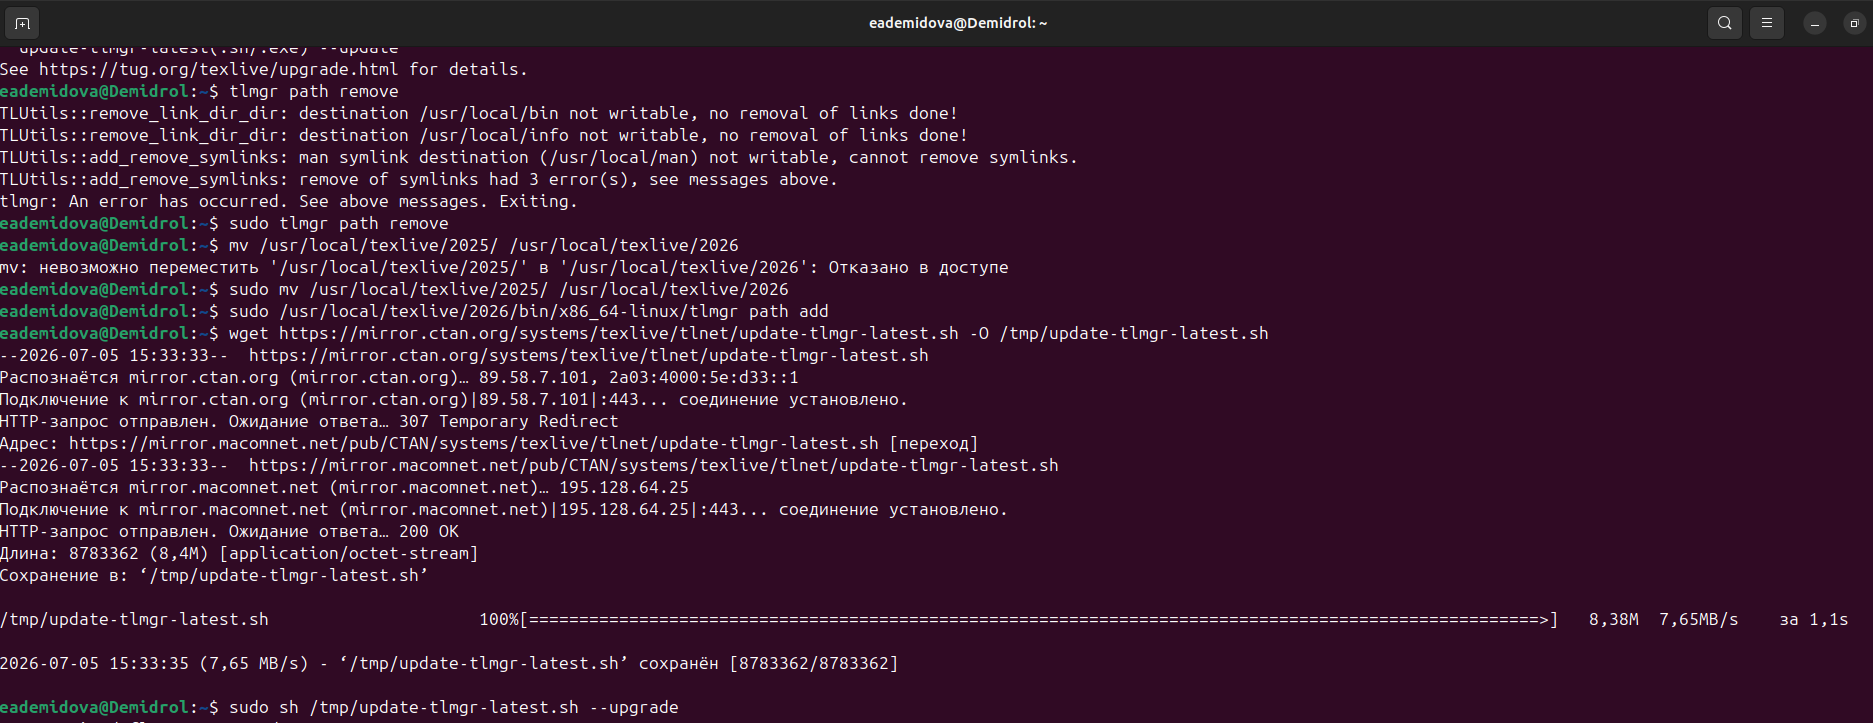
\includegraphics[width=0.7\linewidth,height=\textheight,keepaspectratio]{image/update_script.png}

}

\caption{\label{fig-001}Процесс обновления менеджера пакетов с помощью
скрипта update-tlmgr-latest.sh}

\end{figure}%
\end{frame}

\begin{frame}[fragile]{Обновление всех пакетов}
\protect\phantomsection\label{ux43eux431ux43dux43eux432ux43bux435ux43dux438ux435-ux432ux441ux435ux445-ux43fux430ux43aux435ux442ux43eux432}
После успешного обновления \texttt{tlmgr} была выполнена команда
обновления всех пакетов до актуальных версий:

\begin{Shaded}
\begin{Highlighting}[]
\FunctionTok{sudo}\NormalTok{ /usr/local/texlive/2026/bin/x86\_64{-}linux/tlmgr update }\AttributeTok{{-}{-}self} \AttributeTok{{-}{-}all}
\end{Highlighting}
\end{Shaded}
\end{frame}

\begin{frame}[fragile]{Создание глобальных символических ссылок и
настройка кэша LuaLaTeX}
\protect\phantomsection\label{ux441ux43eux437ux434ux430ux43dux438ux435-ux433ux43bux43eux431ux430ux43bux44cux43dux44bux445-ux441ux438ux43cux432ux43eux43bux438ux447ux435ux441ux43aux438ux445-ux441ux441ux44bux43bux43eux43a-ux438-ux43dux430ux441ux442ux440ux43eux439ux43aux430-ux43aux44dux448ux430-lualatex}
\begin{Shaded}
\begin{Highlighting}[]
\FunctionTok{sudo}\NormalTok{ /usr/local/texlive/2026/bin/x86\_64{-}linux/tlmgr path add}
\end{Highlighting}
\end{Shaded}

Для ускорения работы LuaLaTeX был перенесён кэш шрифтов из старой
версии:

\begin{Shaded}
\begin{Highlighting}[]
\FunctionTok{mv}\NormalTok{ \textasciitilde{}/.texlive2023 \textasciitilde{}/.texlive2026}
\ExtensionTok{luaotfload{-}tool} \AttributeTok{{-}fu}
\end{Highlighting}
\end{Shaded}
\end{frame}

\begin{frame}[fragile]{Проверка итоговой версии}
\protect\phantomsection\label{ux43fux440ux43eux432ux435ux440ux43aux430-ux438ux442ux43eux433ux43eux432ux43eux439-ux432ux435ux440ux441ux438ux438}
Была проверена версия установленного TeX Live:

\begin{Shaded}
\begin{Highlighting}[]
\ExtensionTok{tex} \AttributeTok{{-}{-}version}
\end{Highlighting}
\end{Shaded}

Результат: \texttt{TeX\ 3.141592653\ (TeX\ Live\ 2026)}. Обновление
прошло успешно.
\end{frame}

\begin{frame}{Проверка итоговой версии}
\protect\phantomsection\label{ux43fux440ux43eux432ux435ux440ux43aux430-ux438ux442ux43eux433ux43eux432ux43eux439-ux432ux435ux440ux441ux438ux438-1}
\begin{figure}

\centering{

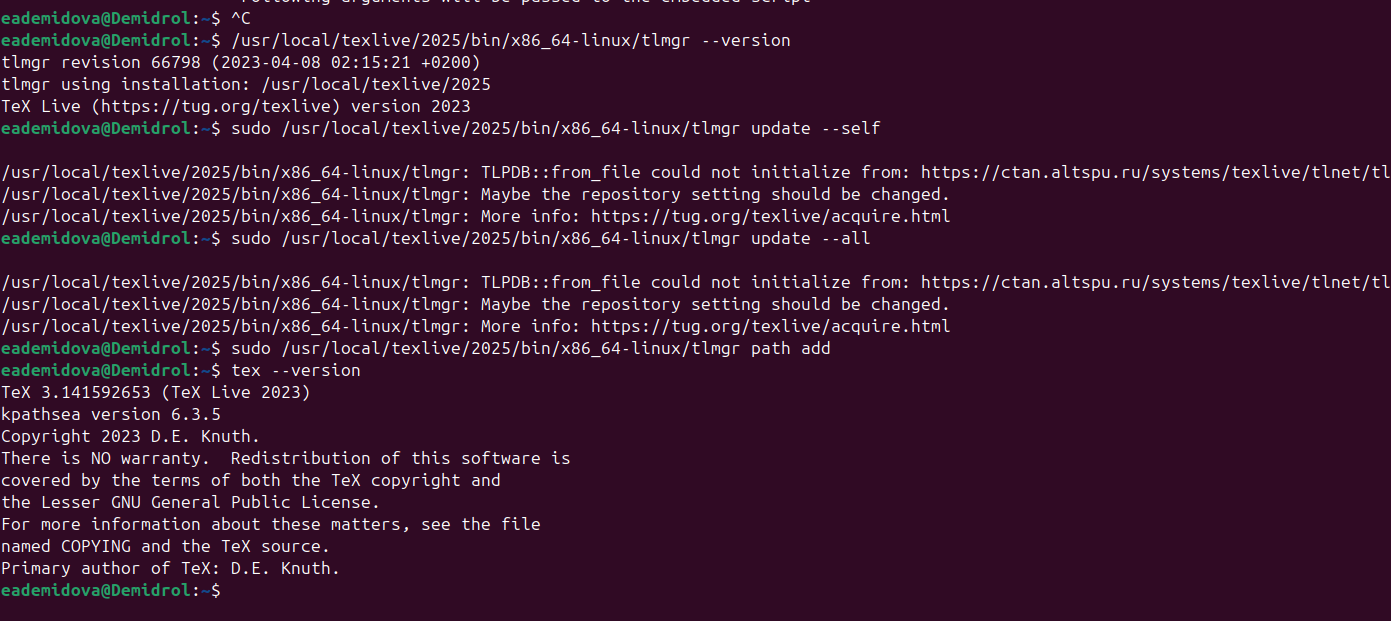
\includegraphics[width=0.7\linewidth,height=\textheight,keepaspectratio]{image/tlmgr_commands.png}

}

\caption{\label{fig-002}Основные команды tlmgr для обновления и
управления пакетами}

\end{figure}%
\end{frame}

\section{Выводы}\label{ux432ux44bux432ux43eux434ux44b}

\begin{frame}[fragile]{Выводы}
В ходе лабораторной работы были получены практические навыки обновления
TeX Live с переходом через несколько мажорных версий. Были использованы
официальные средства (\texttt{update-tlmgr-latest.sh}), а также освоены
команды:

\begin{itemize}[<+->]
\tightlist
\item
  \texttt{tlmgr\ update\ -\/-self} -- обновление менеджера пакетов;
\item
  \texttt{tlmgr\ update\ -\/-all} -- обновление всех установленных
  пакетов;
\item
  \texttt{tlmgr\ path\ add/remove} -- управление символическими
  ссылками;
\item
  \texttt{luaotfload-tool\ -fu} -- обновление кэша шрифтов.
\end{itemize}
\end{frame}

\section{Список
литературы}\label{ux441ux43fux438ux441ux43eux43a-ux43bux438ux442ux435ux440ux430ux442ux443ux440ux44b}

\begin{frame}{Список литературы}
\begin{enumerate}[<+->]
\tightlist
\item
  American Mathematical Society. Why Do We Recommend LaTeX? --- URL:
  https://www.ams.org/publications/authors/tex/latexbenefits ;
  Рекомендации AMS по использованию LaTeX2e. AMS Publications.
\item
  Lamport L. LaTeX: A Document Preparation System. --- 1986. --- Первое
  руководство по LaTeX.
\item
  LaTeX Project. An introduction to LaTeX. --- URL:
  https://www.latex-project.org/about/ ; Дата обращения: 05.07.2026.
  Официальный сайт LaTeX.
\item
  Wikipedia. LaTeX. --- URL: https://en.wikipedia.org/wiki/LaTeX ; Общая
  информация о системе LaTeX. Wikipedia, The Free Encyclopedia.
\end{enumerate}
\end{frame}




\end{document}
